% ============================================================
% 第 1 部分：原 PDF 第 1-16 页
% （第 1 节 作业概览；第 2 节 性能分析与基准测试；
%   第 3 节 单 GPU 内存；第 4 节 GPU 核函数 开头）
% ============================================================

\section{作业概览}

在本次作业中，你将通过动手实践，学习如何提升单 GPU 上的训练速度，以及如何把训练扩展到多块 GPU 上。

\textbf{你要实现的内容}

\begin{enumerate}
  \item 基准测试与性能分析框架（benchmarking and profiling harness）
  \item 激活检查点（activation checkpointing）
  \item FlashAttention 2 的 Triton 核函数（kernel）
  \item 分布式数据并行训练
  \item 优化器状态分片
  \item 完全分片数据并行（fully sharded data parallel）训练
\end{enumerate}

\textbf{代码的结构}

作业代码与这份说明都发布在 GitHub 上：

\begin{center}
\url{github.com/stanford-cs336/assignment2-systems}
\end{center}

请使用 Git 克隆该仓库。如果有任何更新，我们会通知你，届时你可以通过 \tm{git pull} 获取最新版本。

\begin{enumerate}
  \item \tm{cs336-basics/}：在本次作业中，你将对作业 1 中构建的一些组件进行性能分析。该文件夹包含作业 1 的助教参考答案代码，因此你可以在这里找到 \tm{cs336-basics/pyproject.toml} 以及 \tm{cs336-basics/cs336\_basics} 包。如果你想使用自己的模型实现，可以修改根目录下的 \tm{pyproject.toml} 文件，使其指向你自己的包。
  \item \tm{/}：\tm{cs336-systems} 的根目录。我们在其中创建了一个名为 \tm{cs336\_systems} 的空模块。注意这里没有任何代码，所以你完全可以一切从零开始、自行发挥。
  \item \tm{tests/*.py}：该目录包含你必须通过的全部测试。这些测试会调用 \tm{tests/adapters.py} 中定义的钩子（hook）。你需要实现这些适配器（adapter），把你的代码与测试连接起来。多写一些测试和/或修改测试代码对调试很有帮助，但你的实现必须能通过最初提供的测试套件。
  \item \tm{README.md}：该文件包含关于预期目录结构的更多细节，以及一些配置环境的基本说明。
\end{enumerate}

\textbf{如何提交}

你需要向 Gradescope 提交以下文件：

\begin{itemize}
  \item \tm{writeup.pdf}：回答所有笔头问题。请对你的回答进行排版（typeset）。
  \item \tm{code.zip}：包含你编写的全部代码。
\end{itemize}

运行 \tm{test\_and\_make\_submission.sh} 中的脚本即可生成 \tm{code.zip} 文件。

\section{性能分析与基准测试}

在作业的第一部分，我们将探索如何优化 Transformer 模型的性能，以最充分地利用 GPU。我们会先对模型进行性能分析（profiling），了解它在一次前向传播和反向传播过程中把时间和内存花在了哪里；然后用自定义 GPU 核函数（kernel）优化自注意力（self-attention）运算，使其比常规 PyTorch 实现跑得更快。在作业的后续部分，我们将利用多块 GPU，学习如何在集群上训练模型。

\subsection{性能分析}

在实现任何优化之前，最好先对程序做性能分析，弄清楚它把资源（例如时间和内存）花在了哪里。否则，我们可能会去优化那些在时间或内存上并不占大头的部分，从而看不到可衡量的端到端提升。

我们将实现三条性能评估路径：

\begin{enumerate}
  \item 使用 Python 标准库进行简单的端到端基准测试，为前向和反向传播计时；
  \item 使用 NVIDIA Nsight Systems 工具进行计算性能分析，了解这些时间如何分布在 CPU 和 GPU 的各个运算上；
  \item 内存性能分析。
\end{enumerate}

\subsubsection{准备工作：导入你的 basics Transformer 模型}

首先，确认你可以加载上一次作业的模型。在上一次作业中，我们把模型组织成了一个 Python 包，以便后续方便地导入。我们在 \tm{./cs336-basics} 文件夹中加入了模型的参考实现，并在 \tm{pyproject.toml} 文件中指向了它。像往常一样调用 \tm{uv run [command]} 时，uv 会自动找到这个本地的 \tm{cs336-basics} 包。如果你想使用自己的模型实现，可以修改 \tm{pyproject.toml} 文件，让它指向你自己的包。

你可以用如下方式测试能否导入你的模型：

\begin{lstlisting}
$ uv run python
Using CPython 3.13.13
Creating virtual environment at: /path/to/uv/env/dir
        Built cs336-systems @ file:///path/to/systems/dir
        Built cs336-basics @ file:///path/to/basics/dir
Installed 78 packages in 168ms
Python 3.13.13 (main, Apr  7 2026, 20:49:46) [Clang 22.1.1 ] on linux
Type "help", "copyright", "credits" or "license" for more information.
>>> import cs336_basics
...
\end{lstlisting}

作业 1 的相关模块现在应该都可以使用了（例如，对于 \tm{model.py}，可以用 \tm{import cs336\_basics.model} 导入）。

\subsubsection{模型规模}

在整个作业中，我们会对不同规模的模型进行基准测试和性能分析，以更好地理解它们的性能。为了感受规模变化带来的影响，我们将使用并引用下面这些模型配置。除排行榜（leaderboard）中的模型外，其余所有模型我们都使用 10000 的词表大小和 4 的批量大小（batch size），上下文长度则各不相同。本次作业（以及后续作业）需要以表格和图表的形式呈现大量结果。我们强烈建议你用代码自动生成 writeup 中的表格，因为在 LaTeX 或 Typst 中手工排版表格非常繁琐。可以参考 \tm{pandas.DataFrame.to\_latex()} 和 \tm{pandas.DataFrame.to\_typst()}，或者自己编写一个函数，从你偏好的表格表示生成它们。

\begin{table}[htbp]
\centering
\begin{tabular}{@{}lrrrr@{}}
\toprule
规模 & \tm{d\_model} & \tm{d\_ff} & \tm{num\_layers} & \tm{num\_heads} \\
\midrule
small  & 768  & 3072  & 12 & 12 \\
medium & 1024 & 4096  & 24 & 16 \\
large  & 1280 & 5120  & 36 & 20 \\
xl     & 2560 & 10240 & 32 & 32 \\
10B    & 4608 & 12288 & 50 & 36 \\
\bottomrule
\end{tabular}
\caption{不同模型规模的规格说明。这些配置大多基于 GPT-2 的配置。}
\end{table}

除非另有说明，否则使用 512 的上下文长度。

\subsubsection{端到端基准测试}

现在我们来编写一个简单的性能评估脚本。我们要测试模型的许多变体（改变精度、替换层等等），因此让你的脚本能够\textbf{通过命令行参数启用这些变体}会非常值得，方便日后运行。

作为起步，我们先对模型做最简单的性能分析：为前向传播、反向传播和优化器步骤计时。由于我们只测量速度和内存，使用随机的权重和数据即可。

性能测量很微妙——一些常见的陷阱会导致我们测到的并不是想要的量。对 GPU 代码做基准测试时，一个需要注意的地方是 CUDA 调用是\emph{异步}的。当你调用一个 CUDA 核函数（例如调用 \tm{torch.matmul}）时，PyTorch 的函数调用会立即把控制权返回给你的代码，而不会等待矩阵乘法完成。这样，CPU 可以继续抢先运行并调度新的运算，而 GPU 则在一旁完成矩阵乘法，这是一个重要的性能优势。另一方面，这也意味着，天真地测量 \tm{torch.matmul} 调用返回所需的时间，并不能告诉我们 GPU 实际执行矩阵乘法花了多久。在 PyTorch 中，我们可以调用 \tm{torch.cuda.synchronize()} 来等待所有已调度的 GPU 核函数执行完毕，从而更准确地测量 CUDA 核函数的运行时间。这里的同步指的是让 CPU 运行时与 GPU 运行时同步。记住这一点，下面我们来搭建基本的性能分析基础设施。

\subsubsection*{问题（\tm{benchmarking\_script}）：基准测试脚本（4 分）}

\begin{enumerate}[label=(\alph*)]
  \item 编写一个脚本，对模型的前向传播、反向传播和优化器步骤进行基本的端到端基准测试。具体而言，你的脚本应支持以下功能：
  \begin{itemize}
    \item 根据给定的超参数（例如层数），初始化一个模型。
    \item 生成一个随机批次的数据。
    \item 先运行 $w$ 个预热（warm-up）步骤（在开始计时之前），然后为 $n$ 个步骤的执行计时（根据某个参数的取值，可以只做前向、做前向加反向，或者做前向、反向再加优化器步骤）。计时可以使用 Python 的 \tm{timeit} 模块（例如使用 \tm{timeit} 函数，或使用 \tm{timeit.default\_timer()}，它给出系统分辨率最高的时钟，因而比 \tm{time.time()} 更适合作为基准测试的默认选择）。
    \item 在每个步骤之后调用 \tm{torch.cuda.synchronize()}。
  \end{itemize}
  \textbf{交付物：}一个脚本：用给定的超参数初始化一个 basics Transformer 模型，创建一个随机批次的数据，并为仅前向、前向加反向、以及包含优化器步骤的完整训练步骤计时。

  \item 为第 2.1.2 节描述的各模型规模，测量前向、反向和优化器步骤的耗时。使用 5 个预热步骤，并在 10 个测量步骤上计算耗时的平均值和标准差。一次前向传播需要多长时间？反向传播呢？各次测量之间波动很大，还是标准差很小？

  \textbf{交付物：}用 1-2 句话给出你的计时结果。

  \item 基准测试的一个注意事项是要执行预热步骤。在不做预热步骤的情况下重复你的分析。这会如何影响你的结果？你认为为什么会这样？再用 1 或 2 个预热步骤运行脚本试试。为什么结果可能仍然不同？

  \textbf{交付物：}用 2-3 句话回答。
\end{enumerate}

\subsubsection{Nsight Systems 性能分析器}

端到端基准测试无法告诉我们模型在前向和反向传播期间把时间和内存花在了哪里，因而也揭示不出具体的优化机会。要想知道程序在每个组件（例如函数）上花了多少时间，可以使用性能分析器（profiler）。执行分析器通过在函数开始和结束运行处插入探针（guard）对代码插桩，因此可以给出函数级别的详细执行统计信息（例如调用次数、平均耗时、在该函数上累计花费的时间等等）。

标准的 Python 分析器（例如 CProfile）无法分析 CUDA 核函数，因为这些核函数是在 GPU 上异步执行的。幸运的是，NVIDIA 自带一个分析器，可以通过命令行工具 \tm{nsys} 使用。我们建议你通过包管理器获取最新版本，或使用其下载页面提供的安装程序。在作业的这一部分，你将使用 \tm{nsys} 来分析你的 Transformer 模型的运行时行为。

使用 \tm{nsys} 很简单：在前一节的 Python 脚本前面加上 \tm{nsys profile} 运行即可。例如，可以用下面的命令对脚本 \tm{benchmark.py} 做一次基本的分析：

\begin{lstlisting}
$ uv run nsys profile -- python benchmark.py
\end{lstlisting}

然后你可以在本地机器上用 NVIDIA Nsight Systems 桌面应用程序查看分析结果。在分析的 \tm{CUDA API} 行中选中某个特定的 CUDA API 调用（CPU 侧），就会在 \tm{CUDA HW} 行中高亮显示所有相应的核函数执行（GPU 侧）。

一次更全面的分析运行可能如下：

\begin{lstlisting}
$ uv run nsys profile --trace=cuda,cudnn,cublas,osrt,nvtx --pytorch=functions-trace,autograd-shapes-nvtx --cudabacktrace=all --python-backtrace=cuda --gpu-metrics-devices=0 -- python benchmark.py
\end{lstlisting}

\begin{figure}[htbp]
\centering
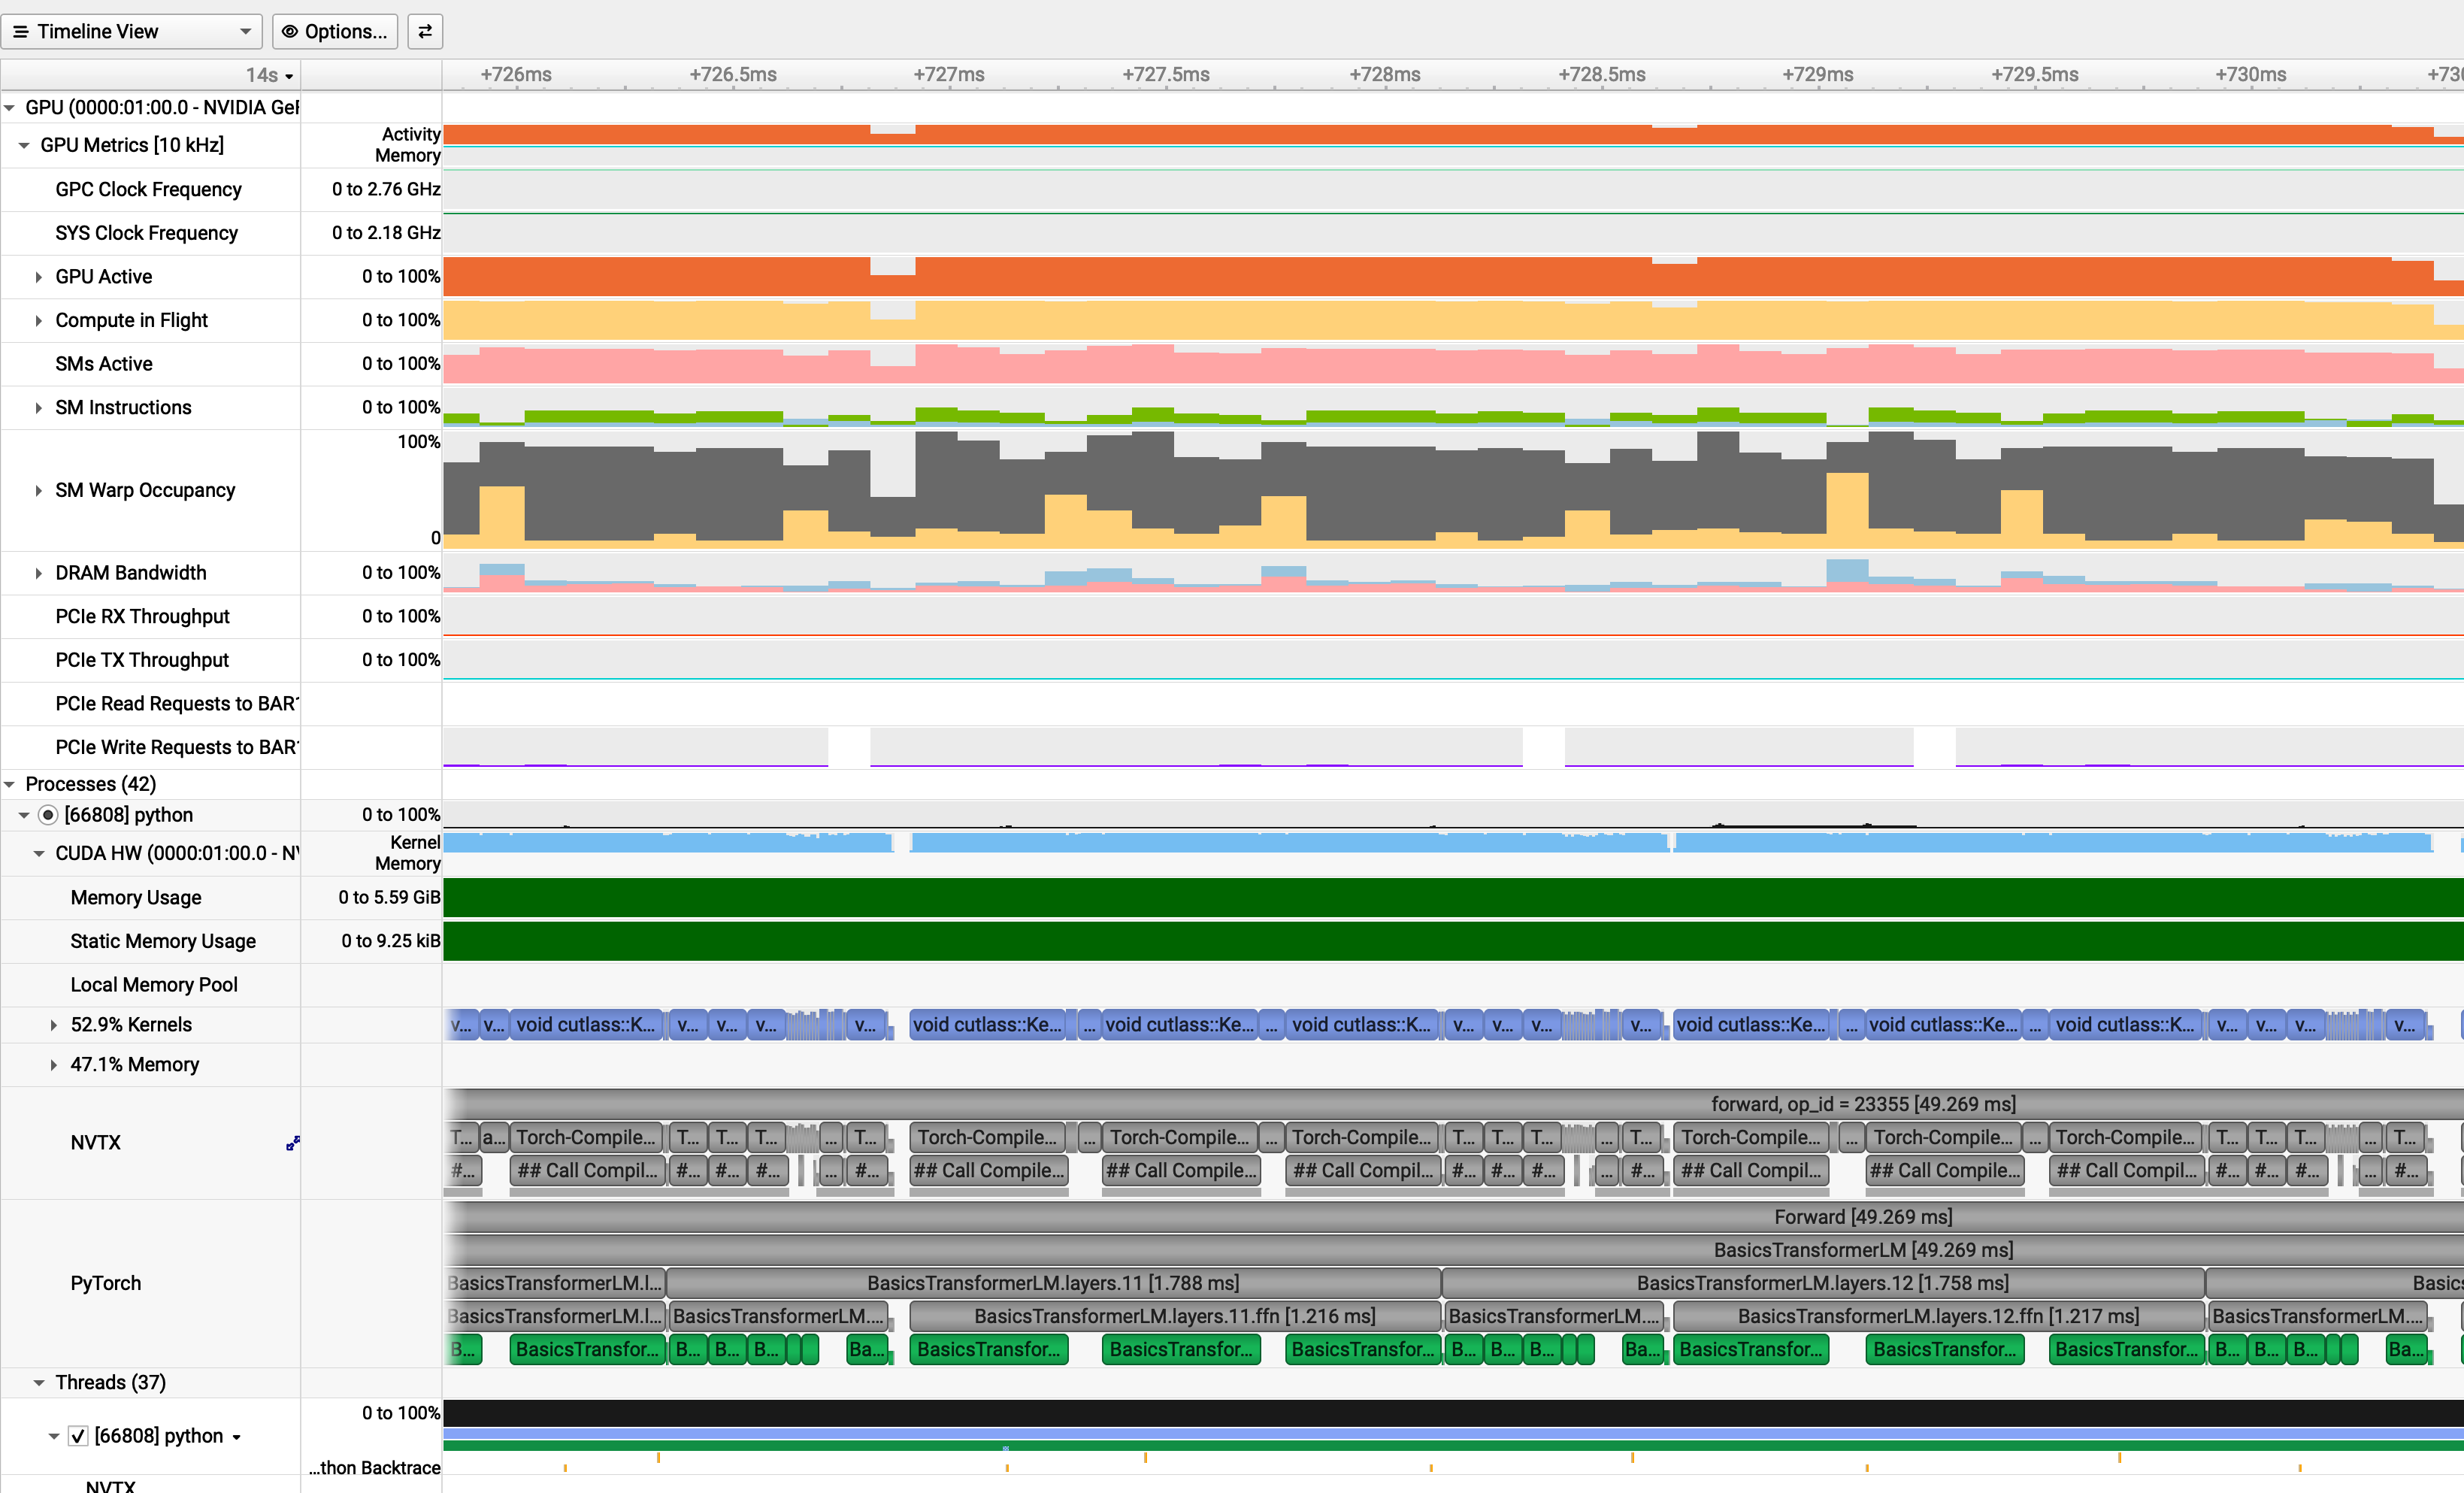
\includegraphics[width=\textwidth]{figures/p05_r05.png}
\caption{一份详细的 Nsight Systems 分析轨迹（trace）}
\end{figure}

在这个例子中，\tm{--trace} 指定要记录哪些 API；\tm{--pytorch} 在模块调用和自动求导期间插入 nvtx 标签；\tm{--cudabacktrace} 和 \tm{--python-backtrace} 提供更好的回溯信息，帮助你了解某个核函数是从代码中的哪里被调用的；\tm{--gpu-metrics-devices} 指定要测量哪块 GPU 的利用率。

为运行添加分析并非没有代价，总体上会拖慢你的运行。通常更可取的做法是只在某次运行中启用你正关注的功能。具体来说，当不需要回溯信息时，你可能想移除 \tm{--cudabacktrace=all} 和 \tm{--python-backtrace=cuda}，因为它们的开销特别大。

我们鼓励你尝试 \tm{nsys profile} 的各种命令行选项，感受一下它能做什么。你还可以用 NVTX 区间（range）标注你的代码，它们会以块的形式出现在分析的 NVTX 行中，涵盖所有 CUDA API 调用及相关的核函数执行。特别地，你应当使用 NVTX 区间来\textbf{忽略基准测试脚本中的预热步骤}（通过对分析中的 nvtx 标签施加 \tm{--nvtx-capture} 过滤器）。你还可以区分出哪些核函数负责模型的前向和反向传播，甚至可以通过如下方式标注你的实现，区分出自注意力层的不同部分分别由哪些核函数负责：

\begin{lstlisting}[language=Python]
...
import torch.cuda.nvtx as nvtx

@nvtx.range("scaled dot product attention")
def annotated_scaled_dot_product_attention(
    ... # Q, K, V, mask
):
    ...
    with nvtx.range("computing attention scores"):
        ... # compute attention scores between Q and K

    with nvtx.range("computing softmax"):
        ... # compute softmax of attention scores

    with nvtx.range("final matmul"):
        ... # compute output projection

    return ...
\end{lstlisting}

在基准测试脚本中，你可以通过下面的方式用带标注的版本替换原来的实现：

\begin{lstlisting}
cs336_basics.model.scaled_dot_product_attention = annotated_scaled_dot_product_attention
\end{lstlisting}

最后值得注意的是，\tm{torch.compile} 会让时间和资源难以归因到代码的特定部分。你可能需要用 \tm{torch.compile} 和 nvtx 标注包裹或剥离代码的各个部分，才能把时间和资源使用正确地归因到源代码的各个部分。

\subsubsection*{问题（\tm{nsys\_profile}）：Nsight Systems 性能分析（5 分）}

使用 \tm{nsys}，从表 1 中自选两个模型规模，以及三个大于 128 的 2 的幂次上下文长度，对你的前向传播、反向传播和优化器步骤进行性能分析，其中可用的最大规模应当是内存能容纳的最长上下文长度。请选择你认为最有意思的组合。对每个分析结果回答以下问题：

\begin{enumerate}[label=(\alph*)]
  \item 你的前向传播总共花了多少时间？这与之前用 Python 标准库测得的结果是否一致？

  \textbf{交付物：}用 1-2 句话回答。

  \item 在前向传播期间，哪个 CUDA 核函数占用最多的累计 GPU 时间？在模型的一次前向传播中，这个核函数被调用了多少次？当你同时做前向和反向传播时，占用运行时间最多的也是同一个核函数吗？（提示：查看 “Stats System View” 下的 “CUDA GPU Kernel Summary”，并利用 NVTX 区间过滤，以确定模型的哪些部分对应哪些核函数。）

  \textbf{交付物：}用 1-2 句话回答。

  \item 尽管绝大多数 FLOPs 都发生在矩阵乘法中，你会注意到还有几个其他核函数也占整体运行时间的相当一部分。在前向传播中，除矩阵乘法外，你还看到哪些核函数占了不可忽视的 CUDA 运行时间？

  \textbf{交付物：}用 1-2 句话回答。

  \item 用你实现的 AdamW 分析一个完整训练步骤的运行（即前向传播、计算损失并运行一次反向传播，最后执行一次优化器步骤，就像训练时那样）。与推理（仅前向传播）相比，花在矩阵乘法上的时间比例有何变化？其他核函数呢？

  \textbf{交付物：}用 1-2 句话回答。

  \item 在前向传播过程中，比较模型自注意力层内 softmax 运算与各矩阵乘法运算的运行时间。运行时间上的差异与 FLOPs 上的差异相比如何？

  \textbf{交付物：}用 1-2 句话回答。
\end{enumerate}

\subsubsection{混合精度}

到目前为止，我们一直以 FP32 精度运行——所有模型参数和激活值都是 \tm{torch.float32} 数据类型。然而，现代 NVIDIA GPU 包含专门用于在低精度下加速矩阵乘法的 GPU 核心（Tensor Core）。例如，NVIDIA B200 的规格表显示其 FP32 最大吞吐量为 80 TFLOPS，而 FP16（半精度浮点数）或 BF16（bfloat16）的最大吞吐量则要高得多，高达 2500 TFLOPS。因此，使用低精度数据类型应当有助于加速训练和推理。

然而，把模型直接转换为低精度格式可能会降低模型的精度。例如，实践中许多梯度值常常小到 FP16 无法表示，于是在用 FP16 精度天真地训练时会变成零。为了解决这个问题，用 FP16 训练时通常会采用损失缩放（loss scaling）——只需把损失乘上一个缩放因子，增大梯度的量级，使其不至于下溢为零。此外，FP16 的动态范围比 FP32 小，可能导致溢出，表现为损失变成 NaN。完整的 bfloat16 训练通常更稳定（因为 BF16 与 FP32 具有相同的动态范围），但与 FP32 相比仍可能影响模型的最终性能。

为了利用低精度数据类型带来的加速，通常会使用\emph{混合精度}（mixed-precision）训练。在 PyTorch 中，它通过 \tm{torch.autocast} 上下文管理器实现。此时，某些运算（例如矩阵乘法）会以低精度数据类型执行，而其他需要 FP32 完整动态范围的运算（例如累加和归约）则保持原样。例如，下面的代码会在前向传播期间自动识别哪些运算应以低精度执行，并把它们转换为指定的数据类型：

\begin{lstlisting}[language=Python]
model : torch.nn.Module = ... # e.g. your Transformer model
dtype : torch.dtype = ... # e.g. torch.bfloat16
x : torch.Tensor = ... # input data

with torch.autocast(device_type="cuda", dtype=dtype):
    y = model(x)
\end{lstlisting}

如上所述，即使被累加的张量本身已经降低精度，通常也最好让累加保持在高精度下进行。下面的练习有助于你建立对此的直觉。

\subsubsection*{问题（\tm{mixed\_precision\_accumulation}）：混合精度累加（1 分）}

运行下面的代码，并对结果的精度加以评述。

\begin{lstlisting}[language=Python]
s = torch.tensor(0,dtype=torch.float32)
for i in range(1000):
    s += torch.tensor(0.01,dtype=torch.float32)
print(s)

s = torch.tensor(0,dtype=torch.float16)
for i in range(1000):
    s += torch.tensor(0.01,dtype=torch.float16)
print(s)

s = torch.tensor(0,dtype=torch.float32)
for i in range(1000):
    s += torch.tensor(0.01,dtype=torch.float16)
print(s)

s = torch.tensor(0,dtype=torch.float32)
for i in range(1000):
    x = torch.tensor(0.01,dtype=torch.float16)
    s += x.type(torch.float32)
print(s)
\end{lstlisting}

\textbf{交付物：}用 2-3 句话回答。

下面我们先把混合精度应用到一个玩具模型上以建立直觉，然后再应用到我们的基准测试脚本中。

\subsubsection*{问题（\tm{benchmarking\_mixed\_precision}）：混合精度基准测试（2 分）}

\begin{enumerate}[label=(\alph*)]
  \item 考虑下面的模型：

\begin{lstlisting}[language=Python]
class ToyModel(nn.Module):
    def __init__(self, in_features: int, out_features: int):
        super().__init__()
        self.fc1 = nn.Linear(in_features, 10, bias=False)
        self.ln = nn.LayerNorm(10)
        self.fc2 = nn.Linear(10, out_features, bias=False)
        self.relu = nn.ReLU()

    def forward(self, x):
        x = self.relu(self.fc1(x))
        x = self.ln(x)
        x = self.fc2(x)
        return x
\end{lstlisting}

  假设我们在 GPU 上训练该模型，且模型参数原本是 FP32。我们想使用 FP16 的自动转型（autocasting）混合精度。下列各项的数据类型分别是什么：

  \begin{itemize}
    \item autocast 上下文内的模型参数？
    \item 第一个前馈层（\tm{ToyModel.fc1}）的输出？
    \item 层归一化（\tm{ToyModel.ln}）的输出？
    \item 模型预测的 logit？
    \item 损失？
    \item 模型的梯度？
  \end{itemize}

  \textbf{交付物：}上面列出的每个组件的数据类型。

  \item 你应该已经看到，FP16 混合精度 autocast 对层归一化层的处理与前馈层不同。层归一化的哪些部分对混合精度敏感？如果用 BF16 代替 FP16，我们还需要区别对待层归一化吗？为什么？

  \textbf{交付物：}用 2-3 句话回答。

  \item 修改你的基准测试脚本，使其可以选择使用 BF16 混合精度运行模型。对第 2.1.2 节描述的每种语言模型规模，分别在使用和不使用混合精度的情况下为前向和反向传播计时。比较全精度与混合精度的结果，并评述模型规模变化时出现的任何趋势。你可能会发现 \tm{nullcontext} 这个空操作上下文管理器很有用。

  \textbf{交付物：}用 2-3 句话给出你的计时结果和评述。
\end{enumerate}

\subsubsection{内存性能分析}

到目前为止，我们关注的是计算性能。现在我们把注意力转向\emph{内存}——语言模型训练和推理中的另一大资源。PyTorch 还自带一个强大的内存分析器，可以跟踪随时间变化的内存分配情况。

要使用内存分析器，可以这样修改你的基准测试脚本：

\begin{lstlisting}[language=Python]
... # warm-up phase in your benchmarking script

# Start recording memory history.
torch.cuda.memory._record_memory_history(max_entries=1000000)

... # what you want to profile in your benchmarking script

# Save a pickle file to be loaded by PyTorch's online tool.
torch.cuda.memory._dump_snapshot("memory_snapshot.pickle")

# Stop recording history.
torch.cuda.memory._record_memory_history(enabled=None)
\end{lstlisting}

这会输出一个 \tm{memory\_snapshot.pickle} 文件，你可以把它加载到在线工具 \url{pytorch.org/memory_viz} 中。该工具让你查看总体内存使用时间线，以及每一次单独的内存分配，包括其大小和指向分配来源代码的栈回溯。要使用该工具，你应在网页浏览器中打开上面的链接，然后把 pickle 文件拖放到页面上。

现在你将使用 PyTorch 分析器来分析自己模型的内存使用情况。

\subsubsection*{问题（\tm{memory\_profiling}）：内存性能分析（4 分）}

对表 1 中的 xl 模型，在上下文长度为 128 和 2048 的情况下，分析其完整训练步骤（前向传播、反向传播和优化器步骤）的内存使用。

\begin{enumerate}[label=(\alph*)]
  \item 在你的分析脚本中添加一个选项，让模型通过内存分析器运行。复用你之前的一些基础设施可能有助于此（例如启用混合精度、加载特定模型规模等）。然后运行脚本，得到 xl 模型在仅推理（只做前向传播）或完整训练步骤时的内存分析结果。你的内存时间线是什么样子？能否根据看到的峰值判断当前正在运行哪个阶段？

  \textbf{交付物：}来自 \tm{memory\_viz} 工具的 xl 模型 “Active memory timeline” 的两张图：一张对应前向传播，另一张对应完整训练步骤（前向和反向传播，然后是优化器步骤），并用 2-3 句话加以说明。

  \item 做前向传播时，每个上下文长度的峰值内存使用是多少？做完整训练步骤时呢？

  \textbf{交付物：}一张表格，每个上下文长度给出两个数字。

  \item 求出 xl 模型在使用混合精度时的峰值内存使用，前向传播和完整训练步骤都要测。混合精度对内存使用有显著影响吗？

  \textbf{交付物：}用 2-3 句话回答。

  \item 考虑 xl 模型。根据我们的参考超参数，Transformer 残差流（residual stream）中的一个激活值张量在单精度下的大小是多少？请用 MiB 给出该大小（即把字节数除以 $1024^2$）。

  \textbf{交付物：}用 1-2 句话给出你的推导。

  \item 现在仔细观察 xl 模型做前向传播的内存快照在 \url{pytorch.org/memory_viz} 上的 “Active Memory Timeline”。当你调低 “Detail” 级别时，工具会隐藏相应级别以下最小的那些分配（例如把 “Detail” 设为 10\% 时，只显示最大的 10\% 的分配）。显示出来的最大分配有多大？通过查看栈回溯，你能说出这些分配来自哪里吗？

  \textbf{交付物：}用 1-2 句话回答。

  \item Nsight Systems 也有用于内存分析的标志。你可以把它们与前面的 Nsight 标志结合使用，以了解模型生命周期的不同步骤中发生了哪些分配。利用 PyTorch 提供的 NVTX 标签，确定模型中单个 \tm{TransformerBlock} 为反向传播保存了多少内存（这些张量常被称为残差，residuals）。记录贡献最大的 5 个运算，以及它们占总体内存的百分比。

  在反向传播期间，所有这些张量都会被释放，但同时会产生新的梯度张量。根据你的分析结果——前向传播期间分配了多少内存，以及反向传播中每经过一个 \tm{TransformerBlock} 内存使用变化多少——计算为一个 \tm{TransformerBlock} 生成的梯度张量占用多少内存。结果与你的预期相符吗？

  \textbf{交付物：}Nsight Systems 的截图以及 1-2 段说明。
\end{enumerate}

\section{单 GPU 内存}

作业的后续部分将探索把张量分片（shard）到多块 GPU 上的技巧，但也有一些技巧即使对单 GPU 训练同样适用。其中最常见的是梯度检查点（gradient checkpointing，也称为激活检查点，activation checkpointing）。

\subsection{自动求导残差}

回顾一下：要对模型执行反向传播，我们需要保存在前向传播中产生的激活值。对某些运算来说这显然是必要的，但默认情况下，会这样做的运算比你预期的多得多。为反向传播保存的张量被称为「残差（residuals）」，或简称「已保存张量（saved tensors）」。

让我们来了解网络中到底保存了什么。从这个不起眼的 RMSNorm 函数开始（为简单起见使用纯 FP32），我们添加一些钩子，在张量被自动求导保存或读取时打印信息。

\begin{lstlisting}[language=Python]
import torch
from torch import nn

x = torch.randn((4, 512, 2560), requires_grad=True)

class RMSNorm(nn.Module):
    def __init__(
        self,
        hidden_size: int,
        eps: float = 1e-5,
        device=None,
    ):
        super().__init__()
        self.weight = nn.Parameter(torch.ones(hidden_size, device=device))
        self.eps = eps

    def forward(self, x):
        rms = torch.rsqrt(x.pow(2).mean(-1, keepdim=True) + self.eps)
        x = x * rms
        return self.weight * x

def pack_hook(t):
    shape, dtype, grad_fn = t.shape, t.dtype, t.grad_fn
    print(f"Saving residual: {shape=}, {dtype=}, {grad_fn=}")
    return t

def unpack_hook(t):
    shape, dtype, grad_fn = t.shape, t.dtype, t.grad_fn
    print(f"Loading residual: {shape=}, {dtype=}, {grad_fn=}")
    return t

ln = RMSNorm(x.shape[-1])

with torch.autograd.graph.saved_tensors_hooks(pack_hook, unpack_hook):
    y = ln(x)
    y.sum().backward()
\end{lstlisting}

输出显示被写出的张量数量多得令人担忧，其中几个还是完整的激活值大小！

\begin{lstlisting}
$ uv run scripts/autograd_experiment.py
Saving residual: shape=torch.Size([4, 512, 2560]), dtype=torch.float32, grad_fn=None
Saving residual: shape=torch.Size([4, 512, 1]), dtype=torch.float32, grad_fn=<RsqrtBackward0 object at 0x7f7dd319b5e0>
Saving residual: shape=torch.Size([4, 512, 1]), dtype=torch.float32, grad_fn=<RsqrtBackward0 object at 0x7f7dd319b5e0>
Saving residual: shape=torch.Size([4, 512, 2560]), dtype=torch.float32, grad_fn=None
Saving residual: shape=torch.Size([4, 512, 2560]), dtype=torch.float32, grad_fn=<MulBackward0 object at 0x7f7dd319b5e0>
Saving residual: shape=torch.Size([2560]), dtype=torch.float32, grad_fn=None

Loading residual: shape=torch.Size([4, 512, 2560]), dtype=torch.float32, grad_fn=<MulBackward0 object at 0x7f7cf14e6740>
Loading residual: shape=torch.Size([2560]), dtype=torch.float32, grad_fn=None
Loading residual: shape=torch.Size([4, 512, 1]), dtype=torch.float32, grad_fn=<RsqrtBackward0 object at 0x7f7cf14e6740>
Loading residual: shape=torch.Size([4, 512, 2560]), dtype=torch.float32, grad_fn=None
Loading residual: shape=torch.Size([4, 512, 1]), dtype=torch.float32, grad_fn=<RsqrtBackward0 object at 0x7f7cf14e6740>
Loading residual: shape=torch.Size([4, 512, 2560]), dtype=torch.float32, grad_fn=None
\end{lstlisting}

\subsubsection{算子融合}

在这个例子中，很明显所用运算的粒度太细了。我们想要一个单一的算子：接收 RMSNorm 权重和激活值，直接给出输出，并且该算子在反向传播中作为一个整体（unitary）来处理。这正是核函数融合（kernel fusion）的动机之一。由于 RMSNorm 的行为相当规范，我们甚至可以用 \tm{torch.compile} 自动融合它。

\begin{lstlisting}[language=Python]
...
ln = torch.compile(RMSNorm(x.shape[-1]))

with torch.autograd.graph.saved_tensors_hooks(pack_hook, unpack_hook):
    y = ln(x)
    y.sum().backward()
\end{lstlisting}

新的输出明显好多了：

\begin{lstlisting}
Saving residual: shape=torch.Size([4, 512, 2560]), dtype=torch.float32, grad_fn=None
Saving residual: shape=torch.Size([2560]), dtype=torch.float32, grad_fn=None
Saving residual: shape=torch.Size([4, 512, 1]), dtype=torch.float32, grad_fn=None
Loading residual: shape=torch.Size([4, 512, 2560]), dtype=torch.float32, grad_fn=None
Loading residual: shape=torch.Size([2560]), dtype=torch.float32, grad_fn=None
Loading residual: shape=torch.Size([4, 512, 1]), dtype=torch.float32, grad_fn=None
\end{lstlisting}

现在我们只需要为反向传播保存一个完整尺寸的激活值张量——即 RMSNorm 函数的输入。还请注意，读取的顺序不再是保存顺序的逆序，而且每个残差也不再带有 \tm{grad\_fn} 依赖——PyTorch 把我们的整个 RMSNorm 当作单个函数来对待。

\subsection{激活检查点}

融合无疑有用，但在节省内存方面它也只能帮我们到这里。例如，我们来把 xl 规模下的单个 \tm{TransformerBlock} 做一下融合。

\begin{lstlisting}[language=Python]
import torch
from cs336_basics.model import RotaryEmbedding, TransformerBlock

# num_layers for this model is 32
d_model, d_ff, num_heads, context_length = 2560, 10240, 16, 2048
block = TransformerBlock(d_model=d_model, d_ff=d_ff, num_heads=num_heads,
positional_encoder=RotaryEmbedding(dim=d_model // num_heads, context_length=context_length))

# Fuse as much torch.compile will allow
block = torch.compile(block, fullgraph=True)
x = torch.randn((4, context_length, d_model), requires_grad=True)
\end{lstlisting}

\begin{lstlisting}[language=Python]
...
# Now logs the number of bytes saved
total_size_bytes = 0
def pack_hook(t):
    if isinstance(t, torch.nn.Parameter):  # Skip logging parameters to avoid double counting
        return t
    global total_size_bytes
    shape, dtype, grad_fn = t.shape, t.dtype, t.grad_fn
    total_size_bytes += t.numel() * t.element_size()
    print(f"Saving residual: {shape=}, {dtype=}, {grad_fn=}")
    return t

...

# Run forward pass, saving for backward
with torch.autograd.graph.saved_tensors_hooks(pack_hook, unpack_hook):
    y = block(x)

print(f"Total size of saved tensors in single TransformerBlock: {total_size_bytes / (1024**2):.2f} MiB")
\end{lstlisting}

这个脚本告诉我们为反向传播保存了多少内存：

\begin{lstlisting}
...
Total size of saved tensors in single TransformerBlock: 3651.31 MiB
\end{lstlisting}

每一层就是 3.6 GiB。如果对所有层都这样做，仅为反向传播而保存的激活值就高达 114 GiB！注意力运算的残差中有相当可观的浪费，我们将在第 4 节修复这个问题；但即使修复之后，内存使用仍会随批量大小、序列长度和嵌入维度线性增长。

\subsubsection{重计算}

我们不必保留生成的每一个张量，而是可以只定期保存结果的检查点，并重新计算中间的值。PyTorch 提供了一个接口，可以用简单的方式处理这件事。\tm{torch.utils.checkpoint.checkpoint} 接收一个函数以及传给该函数的参数，然后按如下方式改变传入函数的行为：

\begin{enumerate}
  \item 在前向传播中：
  \begin{enumerate}
    \item 保存传给该函数的输入值；
    \item 抑制前向传播中张量的保存。
  \end{enumerate}
  \item 在反向传播中：
  \begin{enumerate}
    \item 在前面加上一个重计算步骤：用先前保存的输入重新计算前向传播，并为反向传播保存值；
    \item 运行反向传播，随后所有张量都可以被释放。
  \end{enumerate}
\end{enumerate}

在依次通过 4 个 transformer 块的简单情形中，可以看到内存按我们预期的方式累加。

\begin{lstlisting}[language=Python]
...
def four_blocks(x):
    x = block(x)
    x = block(x)
    x = block(x)
    x = block(x)
    return x

with torch.autograd.graph.saved_tensors_hooks(pack_hook, unpack_hook):
    y = four_blocks(x)

print(f"Total size of saved tensors in four TransformerBlocks: {total_size_bytes / (1024**2):.2f} MiB")
\end{lstlisting}

\begin{lstlisting}
Total size of saved tensors in four TransformerBlocks: 14605.25 MiB
\end{lstlisting}

但我们可以像下面这样采用梯度检查点：

\begin{lstlisting}[language=Python]
from torch.utils.checkpoint import checkpoint
def two_blocks(x):
    x = block(x)
    x = block(x)
    return x

def four_blocks_checkpoint(x):
    # checkpoint throws out all the saved tensors until the backward pass
    # when getting to the checkpointed block in the backward pass,
    # it reruns a forward pass to produce the saved tensors,
    # then completes normal backward pass.
    x = checkpoint(two_blocks, x, use_reentrant=False)
    x = checkpoint(two_blocks, x, use_reentrant=False)
    return x

with torch.autograd.graph.saved_tensors_hooks(pack_hook, unpack_hook):
    y = four_blocks_checkpoint(x)

print(f"Total size of saved tensors in four TransformerBlocks with checkpointing: {total_size_bytes / (1024**2):.2f} MiB")
\end{lstlisting}

\begin{lstlisting}
Saving residual: shape=torch.Size([0]), dtype=torch.float32, grad_fn=None
Saving residual: shape=torch.Size([4, 2048, 2560]), dtype=torch.float32, grad_fn=None
Saving residual: shape=torch.Size([0]), dtype=torch.float32, grad_fn=None
Saving residual: shape=torch.Size([4, 2048, 2560]), dtype=torch.float32,
grad_fn=<torch.autograd.function.CompiledFunctionBackward object at 0x7aa0657a19d0>
Total size of saved tensors in four TransformerBlocks with checkpointing: 160.00 MiB
\end{lstlisting}

请注意，这并没有消除内存使用，而是把我们的内存使用分解成了两类：为在每个 \tm{checkpoint} 调用的入口点准备重计算而保存的较长期存储（即检查点本身），以及在检查点块的重计算过程中产生的短期内存，用于支持穿过该块的反向传播。由于我们主要关心的是峰值内存使用，我们希望取得平衡：一方面是保存检查点的内存开销，另一方面是具体化（materialize）完整一个块的残差的内存开销。使用的检查点越多，单个块内具体化的内存就越少，但检查点本身需要的内存就越多。

在上面我们的例子中，显然重计算残差的内存占了主导（部分原因是我们的检查点非常小），所以把平衡更多地向检查点内存倾斜会更有利。因此，我们会想减小检查点块的范围。

检查点块更大或更小并不影响重计算的计算开销，但我们还可以用\emph{递归检查点}（recursive checkpointing）以计算换内存，即把 \tm{checkpoint} 调用嵌套在其他 \tm{checkpoint} 调用内部。

\subsubsection*{问题（\tm{gradient\_checkpointing}）：内存最优的梯度检查点（4 分）}

考虑一个由 $N$ 个相同块顺序堆叠而成的 Transformer。在不做任何检查点的情况下，全部 $N$ 个块的残差会同时存活，带来 $O(N)$ 的峰值激活内存。我们可以自由地用 \tm{checkpoint} 包裹前向传播的任意子集，包括把 \tm{checkpoint} 调用相互嵌套。

\begin{enumerate}[label=(\alph*)]
  \item 在忽略计算开销的情况下，什么检查点策略能使峰值激活内存最小？描述你会如何安排 \tm{checkpoint} 调用（给出代码示意即可），并给出你的策略的渐近峰值激活内存和计算量关于 $N$ 的函数。假设单个块保存的残差主导了每个检查点的簿记开销。

  \textbf{交付物：}用 3-5 句话描述该策略及其渐近峰值内存，并附一段简短的代码示意。

  \item 考虑上面批量大小为 4、序列长度为 2048 的 xl 模型配置。如果你的时间/计算预算只够做一步重计算（即不能嵌套 \tm{checkpoint} 调用），那么降低峰值内存的最佳检查点策略是什么？对你运行的峰值内存进行性能分析，以验证你的假设。为确保起见，再比较比它小一档和大一档的检查点块大小下的峰值内存。

  \textbf{交付物：}用 3-5 句话描述你的推理，并附上你的策略实测的峰值内存。
\end{enumerate}

\section{GPU 核函数}

\subsection{用 FlashAttention-2 优化注意力}

\subsubsection{PyTorch 注意力基准测试}

你的性能分析结果很可能表明，注意力层在内存和计算两方面都存在优化机会。从高层来看，注意力运算由一次矩阵乘法、随后的 softmax、再一次矩阵乘法构成：

\begin{equation}
\mathrm{Attention}(Q, K, V) = \mathrm{softmax}\!\left(\mathrm{mask}\!\left(\frac{QK^{\top}}{\sqrt{d_k}}\right)\right)V
\end{equation}

朴素的注意力实现需要为每个 batch/head 元素保存形状为 \tm{seq\_len} $\times$ \tm{seq\_len} 的注意力分数矩阵，当序列很长时它会变得非常大，导致任何输入或输出较长的任务出现内存溢出（out-of-memory）错误。我们将按照 FlashAttention-2 论文实现一个注意力核函数：它按分块（tile）计算注意力，从而完全避免显式具体化 \tm{seq\_len} $\times$ \tm{seq\_len} 的注意力分数矩阵，使模型能够扩展到长得多的序列长度。

\subsubsection*{问题（\tm{pytorch\_attention}）：PyTorch 注意力基准测试（2 分）}

\begin{enumerate}[label=(\alph*)]
  \item 在不同规模下对你的注意力实现进行基准测试。编写一个脚本，它将：
  \begin{enumerate}[label=(\roman*)]
    \item 把批量大小固定为 8，不使用多头注意力（即去掉 head 维度）。
    \item 遍历头嵌入维度 $d_{\text{model}}$ 取 \tm{[16, 32, 64, 128]} 与序列长度取 \tm{[256, 1024, 4096, 8192, 16384]} 的笛卡尔积。
    \item 生成相应大小的随机输入 $Q$、$K$、$V$。
    \item 使用这些输入为 100 次注意力前向传播计时。
    \item 测量反向传播开始前已使用的内存量，并为 100 次反向传播计时。
    \item 记得预热，并在每次前向/反向传播后调用 \tm{torch.cuda.synchronize()}。
  \end{enumerate}

  取决于你的 GPU，其中某些配置预计会发生内存溢出。报告这些配置下你得到的计时结果（或内存溢出错误）。在什么规模下会出现内存溢出错误？对你找到的溢出配置中最小的一个，核算注意力的内存使用（可以使用作业 1 中关于 Transformer 内存占用的公式）。为反向传播保存的内存随序列长度如何变化？你会怎么做来消除这部分内存开销？

  \textbf{交付物：}一张包含计时结果和内存使用计算的表格，以及 1-2 段说明。
\end{enumerate}

\subsection{JIT 编译注意力的基准测试}

从 2.0 版本起，PyTorch 还自带一个强大的即时（just-in-time）编译器，它会自动尝试对 PyTorch 函数应用多种优化：入门介绍参见 \url{https://pytorch.org/tutorials/intermediate/torch_compile_tutorial.html}。特别是，它会通过动态分析你的计算图，尝试自动生成融合的 Triton 核函数。使用 PyTorch 编译器的接口非常简单。例如，如果想把它应用于模型中的单个层，可以这样写：

\begin{lstlisting}[language=Python]
layer = SomePyTorchModule(...)
compiled_layer = torch.compile(layer)
\end{lstlisting}

现在，\tm{compiled\_layer} 在功能上的表现与 \tm{layer} 完全一样（包括它的前向和反向传播）。我们也可以用 \tm{torch.compile(model)} 编译整个 PyTorch 模型，甚至编译调用了 PyTorch 运算的 Python 函数。

\subsubsection*{问题（\tm{torch\_compile}）：Torch Compile（2 分）}

\begin{enumerate}[label=(\alph*)]
  \item 扩展你的注意力基准测试脚本，加入你的 PyTorch 注意力实现的一个编译版本，并在与上文 \tm{pytorch\_attention} 问题相同的配置下，比较编译版本与未编译版本的性能。
\end{enumerate}
